\documentclass[12pt,a4paper]{article}

\usepackage[utf8]{vietnam}
\usepackage{graphicx}
\usepackage{hyperref}
\usepackage{fixltx2e}
%\usepackage{fancybox}
\usepackage[left=3.50cm, right=2.00cm, top=2.00cm, bottom=2.00cm]{geometry}

\hypersetup{
    colorlinks=true,
    linkcolor=blue,
    filecolor=magenta,      
    urlcolor=cyan,
    pdftitle={Sharelatex Example},
    bookmarks=true,
    pdfpagemode=FullScreen,
}

\begin{document}
	\thispagestyle{empty}

	\begin{center}
		\begin{large}
			TRƯỜNG ĐẠI HỌC BÁCH KHOA HÀ NỘI
		\end{large} \\
		\begin{large}
			VIỆN CÔNG NGHỆ THÔNG TIN VÀ TRUYỀN THÔNG
		\end{large} \\
		\textbf{--------------------  *  ---------------------}\\
		
		\begin{figure}[h!]
			\begin{center}
				\includegraphics[width=0.2\linewidth]{logoBK.png}
			\end{center}	
		\end{figure}
		
		{\fontsize{32pt}{1}\selectfont BÁO CÁO MÔN HỌC}\\
		{\fontsize{20pt}{1}\selectfont TÍNH TOÁN PHÂN TÁN}\\[5cm]
	\end{center}

	\hspace{5cm} Sinh viên thực hiện : \hspace{4pt}
	\textbf{\parbox[t]{5cm}{    
		Nguyễn Bình Minh
	}}\\[12pt]

	\hspace{5cm} MSSV \hspace{20pt} : \hspace{4pt} \textbf{\parbox[t]{5cm}{    
		 20152453
	}}\\[12pt]

	\hspace{5cm} GV hướng dẫn \hspace{20pt} :  \hspace{2pt} \textbf{\parbox[t]{5cm}{    
		TS. Đào Thành Chung
	}}

	\vspace{3cm}
	\begin{center}	
		{\fontsize{16pt}{1}\selectfont HÀ NỘI}\\
		{\fontsize{16pt}{1}\selectfont \today}
	\end{center}
	\newpage
	\pagenumbering{gobble}
		\tableofcontents
	\pagenumbering{arabic}
	\section{Cơ chế đồng thuận}
	Cơ chế đồng thuận Proof-of-Stake Voting (PoSV) là giao thức Proof-of-Stake (PoS) cơ bản với cơ chế bỏ phiếu công bằng
	\section{Kiến trúc TomoChain}
	Kiến trúc chuỗi TomoChain duy trì một tập các masternodes trong sự nhất quán thông qua giao thức đồng thuận TomoChain. 
	\begin{itemize}
		\item Coin-holder (người nắm giữ TOMO) phải giữ ít nhất 1 lượng coin tối thiểu được yêu cầu để trở thành masternode.
		\item Các ứng viên sẽ nhận phiếu bầu từ phía coin-holder.
		\item Những ứng viên nhận được nhiều phiếu bầu nhất sẽ được lựa chọn trở thành Masternodes.
		\item Việc tạo block sẽ được xoay vòng và luân chuyển đi kèm với cơ chế đồng thuận hai lớp.
		\item Masternode sau khi tiến hành việc tạo và xác thực block sẽ được nhận thưởng.
	\end{itemize} 
	TomoChain với kĩ thuật mới gọi là Double Validation với cơ chế Randomization.  Kĩ thuật mới này làm giảm đáng kể xác suất có chuỗi không hợp lệ trong blockchain.

	\section{Election Leader}
	\subsection{Coin-holders, Masternodes}
		\paragraph{Coin-holder}
		 là những người dùng join vào mạng , mà sở hữu và chuyển giao TOMO.
		\paragraph{Masternodes}
		là fullnodes mà duy trì một bản copy của blockchain, tạo những blocks và giữ cho chuỗi nhất quán.
		Masternodes được chọn thông qua hệ thống bầu cử. 
		\begin{itemize}		
			\item Yêu cầu đặt cọc để trở thành một ứng viên chạy masternode là 50.000 TOMO
			\item Những ứng cử viên này sẽ được liệt kê trên Voting DApp, cho coin-holders bầu họ bằng cách gửi TOMO tới smart contract.
		\end{itemize}
		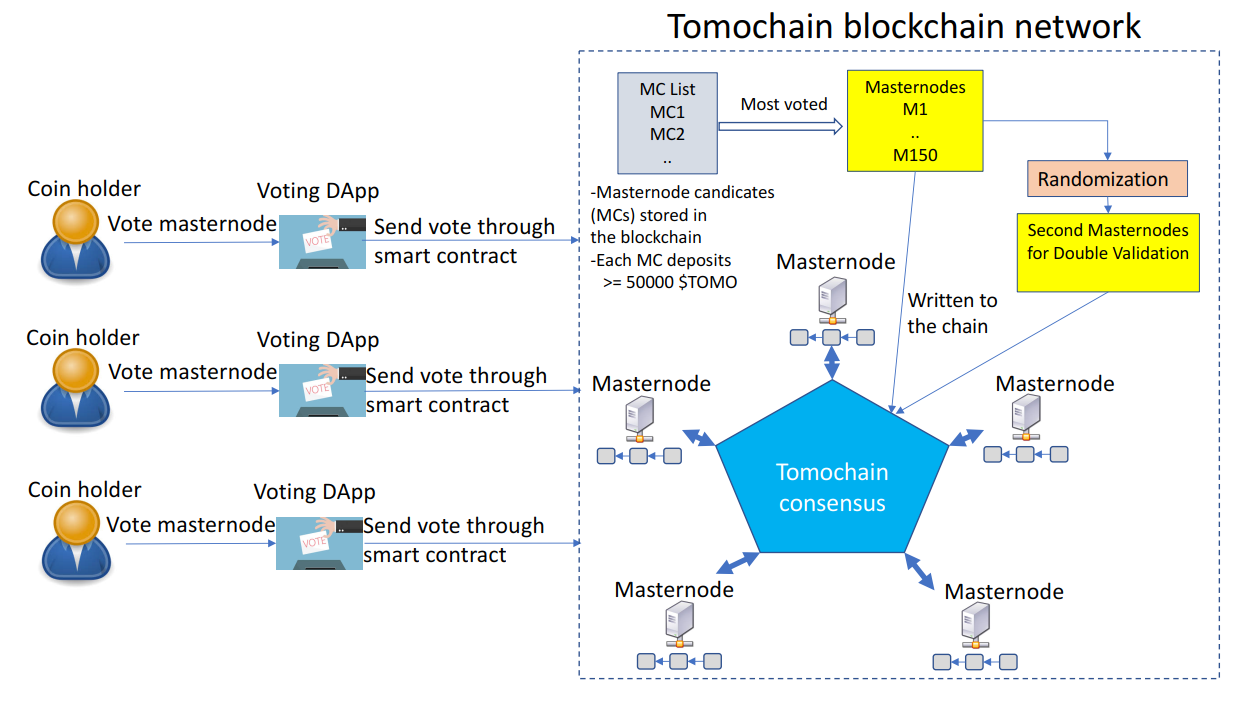
\includegraphics[width=\linewidth]{tomoarchitec.png} \\
	\subsection{Bầu chọn (Voting)}		
		\subparagraph{} Những masternode làm việc chăm chỉ để tạo và xác nhận khối trong hệ thống sẽ được khuyến khích bằng việc tặng TOMO. Hơn nữa, những người nắm giữ token mà bầu chọn cho các masternode này cũng sẽ nhận TOMO theo tỷ lệ lượng TOMO mà họ đã đầu tư cho các masternode qua việc bầu chọn. Các kỹ sư của TomoChain có nhiệm vụ thiết kế ra một cơ chế thưởng công bằng, minh bạch, tự động và dễ tính toán. 
		\subparagraph{} Việc bầu chọn được coi như lượng đầu tư của họ cho những masternode họ ủng hộ. Hay một chiến lược bầu chọn giúp tối đa lợi nhuận của họ. Do đó, masternodes luôn phải chạy đua để có vị trí tốt hơn.
		\subparagraph{} Danh sách các ứng viên masternode sẽ được chọn lọc liên tục dựa vào lượng token bầu chọn. Hiệu quả hoạt động của các masternode sẽ được theo dõi và báo cáo ngược lại cho những người nắm giữ token theo 3 thông số sau: CPU, bộ nhớ và số khối được kí thể hiện hiệu suất của họ. Khối được kí cuối cùng cũng chỉ ra hoạt động cuối cùng của một masternode. Có tối đa 150 ứng viên được chọn để trở thành masternode.
	\subsection{Cơ chế thưởng (Reward Mechanism)}
		\subparagraph{} Mỗi epoch bao gồm 900 khối, tương đương với phần thưởng là 250 TOMO trong hai năm đầu tiên. Lượng 250 TOMO này sẽ được chia cho tất cả các masternode theo tỷ lệ số chữ kí mà họ kí trong một epoch. Sau đó, phần thưởng kiếm được bởi mỗi masternode sẽ được chia thành 3 phần:
		 \begin{itemize}		
			\item Phần thưởng cho cơ sở hạ tầng: 40 \%, sẽ được chuyển cho người sở hữu masternode.
			\item Phần thưởng staking: 50 \% sẽ được chuyển cho nhóm những người bầu chọn cho masternode.
			\item Phần thưởng cho tổ chức sáng lập: 10 \% còn lại được kiểm soát bởi tổ chức sáng lập của Masternode (TomoChain)
		\end{itemize}
		
	
	\section{TomoChain Consensus Protocol}
		\subsection{Double Validation Process}
		Xác thực hai lớp trong TomoChain yêu cầu chữ ký của 2 masternode trong một block để có thể thêm vào blockchain là \textbf{block creator} (block producer) và \textbf{block verifier} chọn ngầu nhiên trong các masternode được đã bầu.  
		\begin{center}
			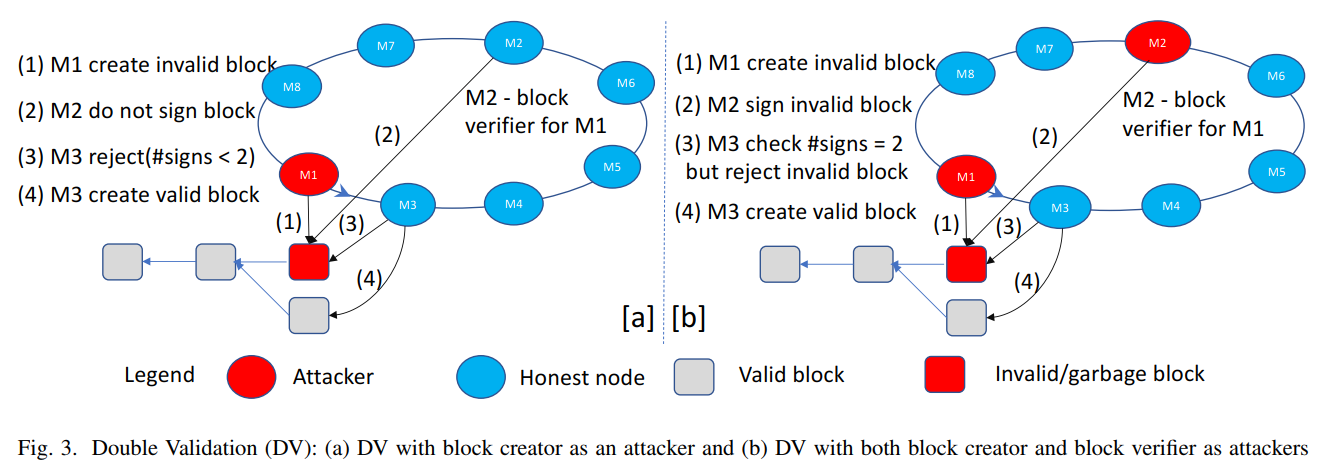
\includegraphics[width=\linewidth]{DV.png} 
		\end{center}
		Nếu M2 là kẻ tấn công bắt tay với M1 kí  (sign) block100 mặc dù nó là invalid
		\begin{itemize}		
			\item Single validation: M2 sau đó  tạo block101 là valid, M3 sẽ kí block101 . Khi đó phải 'rebase' để khôi phục tính hợp lệ của blockchain 
			\item Double validation: M3 lúc này sẽ từ chối (reject) block101 do không đủ 2 chữ kí
		\end{itemize}


		\subsection{Algorithm}
		Một số kí hiệu và định nghĩa
		\begin{itemize}		
			\item Mỗi epoch gồm n (900) block slot,mỗi slot chỉ được tạo 1 block: e\textsubscript{1} <-- \{ sl\textsubscript{1}, sl\textsubscript{2}, ... , sl\textsubscript{n} \}
			\item Có tập gồm m (150) masternotes tương tác thông qua giao thức để đạt sự thống nhất: VC <-- \{ V\textsubscript{1}, V\textsubscript{2}, ... , V\textsubscript{m} \}
			\item Mỗi masternode V\textsubscript{i} có một cặp public/private key ( pk\textsubscript{i}, sk\textsubscript{i} ) và giả sử đều biết public key của những node khác.
			\item Block B\textsubscript{j} tạo tại slot sl\textsubscript{i} gồm state st\textsubscript{i} = Hash(
B\textsubscript{j-1}) , dữ liệu d , chữ ký Sign\textsubscript{sk\textsubscript{i}} ( st, d, sl\textsubscript{i})		
		\end{itemize}
		\begin{center}
			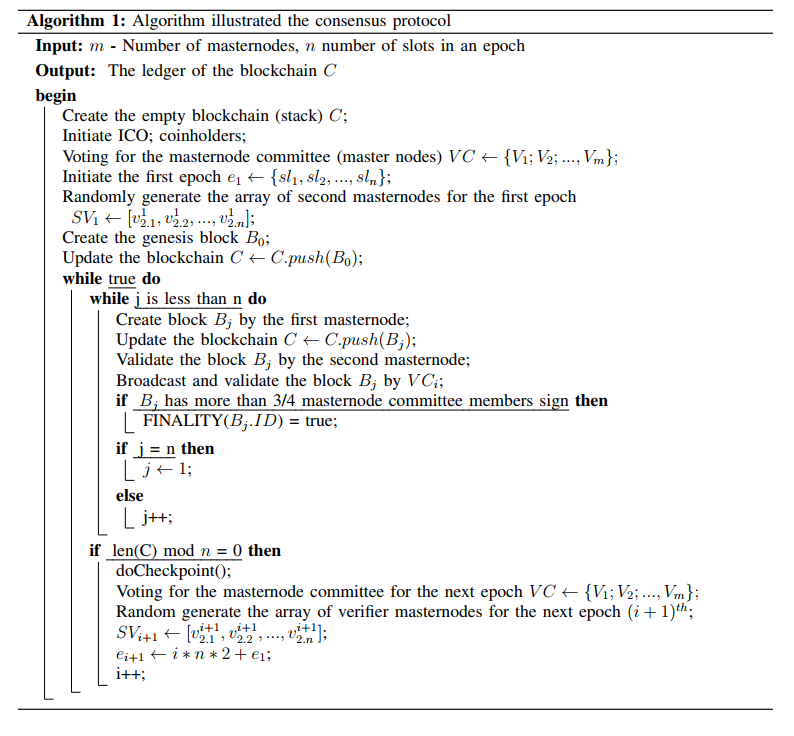
\includegraphics[width=\linewidth]{algo.png} 
		\end{center}

		\subsection{Sharding}
		Thay vì từng masternode lưu trữ tất cả blockchain, thì từng node chỉ cần lưu trữ một phần của nó.
		TomoChain sử dụng 150 masternodes để tạo blocks và bảo mật mạng. Mỗi epoch, ngẫu nhiên chia 10-15 masternode mỗi shard.
		Consensus Smart Contracts:
		\begin{itemize}		
			\item Voting Smart Contract
			\item Block Signer Smart Contract
		\end{itemize}
		Có một root chain tương tác với shard chain. Root chain được sử dụng chủ yếu để đảm bảo giao dịch trong từng shard nhưng không lưu trữ chi tiết giao dịch. Block tạo ra được công nhận nếu 3/4 trong tổng số masternode trong shard đó xác minh và kí trên đó.
		\begin{center}
			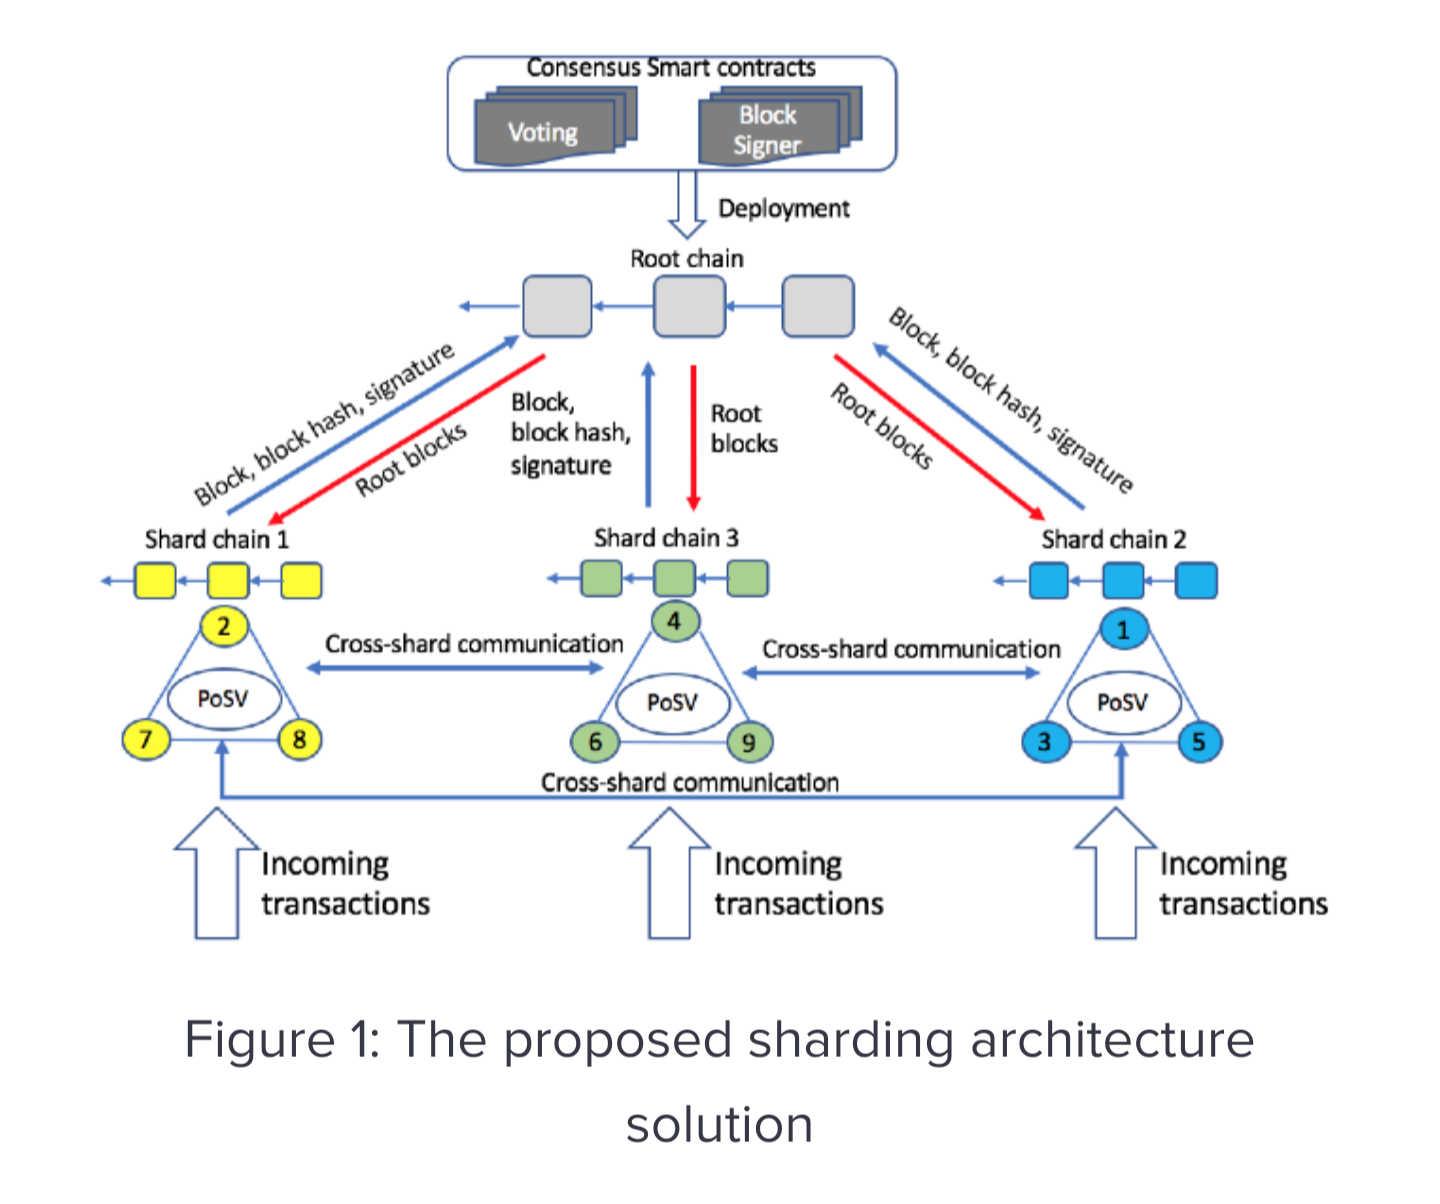
\includegraphics[width=\linewidth]{sharding.png} 
		\end{center}

\end{document}